\chapter{Методология создания DSM-решения}
В данной главе рассматриваются основные этапы жизненного цикла визуального предметно-ориентированного 
языка и рассматриваются возможности по автоматизации каждого этапа. Описывается "`классическая"' 
методология создания визуального языка с использованием метаредактора и методология 
"`метамоделирования на лету"'. Формулируются требования к средствам инструментальной 
поддержки, реализация этих требований в системе QReal будет описана в главе~\ref{chapterImplementation}.

\section{Фазы жизненного цикла визуального предметно-ориентированного языка}
Визуальные предметно-ориентированные языки, как и все искусственные языки, создаются, 
развиваются, устаревают и выводятся из эксплуатации. В случае с предметно-ориентированными 
языками эти процессы проходят относительно быстро, и часто повторяются, нередко случается 
так, что язык создаётся и развивается вместе с решением той задачи, для которой предназначен. 
Поэтому для предметно-ориентированных языков понимать их жизненный цикл особенно важно, 
чтобы иметь возможность организовать процесс их массового создания и поддержки. Исходя 
из проведённого анализа методологий и собственного опыта, будем выделять следующие 
этапы жизненного цикла предметно-ориентированных языков.

\begin{enumerate}
	\item Анализ применимости. 
	\item Анализ предметной области.
	\item Проектирование и реализация.
	\item Развёртывание.
	\item Эволюция языка.
	\item Вывод из эксплуатации.
\end{enumerate}

Данные этапы не обязательно проходятся последовательно, более типична ситуация, когда 
разработка языка ведётся итеративно. Кроме того, возможно даже перекрытие деятельностей, 
ведущихся в разных фазах, так что между фазами часто нет чётких границ. Представленные 
фазы жизненного цикла общие для всех предметно-ориентированных языков (в том числе 
и текстовых), конкретная последовательность фаз, через которую проходит проект, определяется 
моделью жизненного цикла, которая будет введена позже, при описании методологии. Кроме 
того, видно, что жизненный цикл предметно-ориентированного языка рассматривается здесь 
в тесной связи с жизненным циклом использующего его предметно-ориентированного решения --- 
существуют языки, живущие независимо от реализующих их инструментов (в том числе и 
предметно-ориентированные языки, такие как SQL), но в данной работе такие языки не 
рассматриваются. Реализация предметно-ориентированного решения для уже разработанного 
языка, как и разработка языка без разработки инструментальных средств его поддержки, 
являются частными случаями более общей задачи разработки DSM-решения целиком, и достаточно 
нетипичны, чтобы их можно было отдельно не рассматривать.

Некоторые исследователи разделяют фазы проектирования и реализации, а также выделяют 
в отдельную фазу стабилизацию решения. Несмотря на то, что по нашему опыту решение 
может находиться в фазе стабилизации годами, мы будем считать её частью фазы проектирования 
и реализации, поскольку трудно разделить деятельности, ведущиеся на этих этапах. Сами 
проектирование и реализацию также, как представляется, не следует разделять, поскольку 
при использовании DSM-платформы довольно большая часть реализации может быть создана 
автоматически по результатам проектирования (как правило, метамодели).

Ниже приводится описание основных деятельностей, проводимых на каждом этапе, и соображения 
по поводу возможности их автоматизации.

\subsection{Анализ применимости}
\label{chapterFeasibilityStudy}
На этом этапе имеется задача, к которой может быть применён предметно-ориентированный 
подход, однако неясно, насколько оправдано его применение. Задачей фазы анализа применимости 
является оценка всех факторов, которые могут оказать влияние на успешность применения 
предметно-ориентированного решения, и вынесение решения о целесообразности начала 
его разработки. Среди таких факторов наиболее важными являются следующие.

Наличие достаточно узкой предметной области, и наличие повторяющихся задач в ней, 
либо же задачи с большим количеством необходимых для её решения повторяющихся действий.

Наличие экспертизы в предметной области.  Перед тем, как создавать своё DSM-решение, 
как правило, желательно реализовать несколько проектов в предметной области вручную. 
В любом случае, в разработке должен участвовать человек, обладающий достаточно полным 
представлением о предметной области.

Наличие команды высококвалифицированных программистов, которые будут заниматься разработкой 
самого предметно-ориентированного решения. Ошибки и недоделки в инструментальных средствах 
решения будут проявляться во всех проектах, выполненных с помощью этого решения, поэтому 
для разработки требуется привлекать по возможности лучших профессионалов.

Наличие необходимых ресурсов и поддержки со стороны руководства. Создание предметно-ориентированного 
решения сопряжено с довольно высоким уровнем риска и является в некотором смысле долгосрочной 
инвестицией --- преимущества от его внедрения проявятся только через некоторое (иногда 
довольно значительное) время. Кроме того, внедрение предметно-ориентированного решения 
может привести к изменениям в структуре и в бизнес-процессах компании, руководство 
должно быть к этому готово.

Эта фаза наиболее сложна в автоматизации. Оценка должна быть выполнена экспертом на 
основании собственного опыта и слабоформализуемых знаний. Могут помочь рекомендации 
и анкета, приведённые в \cite{kelly2008domain}, эта (или подобная) анкета также может 
быть реализована в каком-либо инструменте, но каждый проект имеет слишком много особенностей, 
чтобы их можно было учесть и предоставить авторам DSM-решения содержательную помощь. 
Кроме того, обычно если авторы уже начали пользоваться каким-либо инструментом, решение 
о начале проекта уже принято. Таким образом, неудивительно, что фаза анализа применимости 
не автоматизирована ни в одном из известных нам инструментов.

\subsection{Анализ предметной области}
\label{chapterDomainAnalysis}
На данном этапе используется опыт экспертов предметной области, чтобы выделить ключевые 
сущности создаваемого языка и отношения между ними. Существует ряд формальных методологий 
анализа, таких как FAST, FODA
% TODO: Ссылки
, и другие. Однако такие методологии используются довольно 
редко (поскольку, как правило, ресурсоёмки, и подходят только для больших проектов), 
чаще используются более неформальные подходы. Некоторые указания по этому поводу можно 
найти в \cite{mernik2005and}, \cite{voelter2009best}, \cite{luoma2004defining} и опять 
же в \cite{kelly2008domain}. Следует отметить, что в данном случае методы, применимые 
для текстовых языков, могут быть перенесены на визуальные языки без изменений, поскольку 
подходы к анализу предметной области мало зависят от последующей реализации языков. 
Результатом этой фазы должна стать концептуальная модель предметной области, включающая 
в себя основные сущности (которые потом станут сущностями создаваемого визуального языка), 
атрибуты этих сущностей, связи между сущностями. Кроме того, может быть полезно составить 
словарь предметной области и описание общих и отличающихся частей создаваемого продукта 
(или линейки программных продуктов), для разработки которого создаётся предметно-ориентированный 
язык.

Кратко перечислим методы анализа предметной области здесь.
\begin{enumerate}
	\item Предметно-ориентированные визуальные языки часто строятся над существующей 
		библиотекой. В таком случае концепции можно брать напрямую из существующего кода.
	\item Эксперты предметной области могут уже иметь средства выражения знаний предметной 
		области, имеют свой профессиональный язык, но не имеют инструментов для формализации 
		своих знаний. Часто употребляемые экспертом в разговоре существительные могут 
		стать сущностями, реже употребляемые существительные --- атрибутами сущностей, 
		глаголы --- операциями или связями. 
	\item Если язык призван визуализировать аппаратную систему, то хорошие кандидаты 
		для сущностей --- физические компоненты.
	\item Хорошим источником сущностей может служить пользовательский интерфейс системы.
	\item Бывает полезно проанализировать пространство изменчивости предметной области 
		(variability space), тогда язык может визуализировать изменяющиеся её части, а 
		постоянные части будут реализованы в виде предметно-ориентированной библиотеки, 
		или фиксированы в генераторе. Такой подход наиболее уместен при разработке линейки 
		программных продуктов.
\end{enumerate}

Инструментальная поддержка фазы анализа может быть весьма развитой, но, как отмечается 
авторами \cite{mernik2005and}, существующие инструменты такой поддержкой не обладают, 
оставляя её специализированным инструментам инженерии знаний. Различные методологии 
анализа предметной области требуют различных инструментов (например, для FODA нужен 
визуальный язык описания требований, для анализа знаний экспертов достаточно обычной 
ER-диаграммы). Наличие таких инструментов в DSM-платформе может существенно облегчить 
и упорядочить сбор и анализ сведений о предметной области, тем более потому, что это 
делается всё равно, но неформально, или формальными средствами, для этого не предназначенными. 
По результатам анализа возможно автоматически генерировать прототип метамодели языка, 
можно организовать трассировку между метамоделью и моделью предметной области, давая 
возможность отслеживать, как изменения в наших знаниях о предметной области отразятся на метамодели.

Проект QReal ориентирован на "`легковесный"' процесс создания предметно-ориентированных 
языков и предназначен для небольших и средних проектов, поэтому инструментальная поддержка 
формального анализа предметной области, хотя и является важной и интересной темой, 
выходит за рамки данной работы. В QReal предлагается новый подход к анализу предметной 
области, совмещённому с созданием прототипа метамодели и одновременно с тестированием языка, 
подробнее об этом в разделе~\ref{chapterMetamodelingOnFly} Возможно, другие виды анализа будут реализованы 
в QReal в дальнейшем.

\subsection{Проектирование и реализация}
Проектирование и реализация визуального языка --- наиболее хорошо изученная и поддержанная 
в существующих инструментах фаза его жизненного цикла. Помимо описания самого языка, 
обычно требуется реализовать визуальный редактор для него, генератор, предметно-ориентированную 
библиотеку, другие инструментальные средства (подробнее о составляющих DSM-решения и 
соображениях по их реализации см. в \cite{kelly2008domain}). На этой фазе опыт разработки 
текстовых языков оказывается неприменим, поскольку текстовые языки обычно задаются с 
помощью грамматик, а визуальные языки --- с помощью метамоделей.

Типичная деятельность по проектированию и реализации визуального языка включает в себя 
формализацию абстрактного синтаксиса создаваемого языка (в подавляющем большинстве случаев 
с помощью метамодели), задание конкретного синтаксиса, автоматическая генерация по этим 
описаниям редактора языка, описание в том или ином виде семантики языка. Как правило, 
задаётся денотационная семантика путём создания генератора из моделей на визуальном языке 
в какой-либо текстовый язык, но возможно и задание правил интерпретации языка (в том числе, 
в виде операционной семантики, как набора правил преобразования моделей). При использовании 
генеративного подхода типичные деятельности включают в себя написание модельного приложения, 
в которое будет производиться генерация из визуального языка "`вручную"', разработка генератора, 
разработка предметно-ориентированной библиотеки, с которой будет работать сгенерированный код. 
По техническим вопросам реализации существует большое количество литературы, поэтому 
не будем останавливаться на них подробно.

Отдельный интересный вопрос, который зачастую обходится в работах по реализации предметно-ориентированных 
визуальных языков, и часто упоминается в работах по реализации языков текстовых --- переиспользование 
синтаксиса существующих языков. Как и в случае с текстовыми языками, визуальный язык 
вовсе не обязательно создавать с нуля, можно использовать уже существующие языки и 
использовать их как базу для создаваемого, путём создания "`лёгких"' расширений (например, 
с помощью механизма профилей UML), либо путём переиспользования и расширения частей 
существующих метамоделей. Существующие технологии имеют тенденцию поощрять создание DSL с нуля, 
это не всегда оптимально. А чтобы поддержать переиспользование метамоделей, в DSM-платформе 
должны наличествовать специальные средства, такие как просмотрщики метамоделей, возможность 
декомпозиции метамодели и импорта.

Требования к инструментальной поддержке фазы реализации подробно описаны в литературе 
(например, в \cite{kelly2008domain}). Тут укажем лишь те требования, которые были 
положены в основу проекта QReal.

\begin{enumerate}
	\item Наличие визуального языка описания метамодели и визуального редактора конкретного 
		синтаксиса языка (редактора формы фигур).
	\item Наличие возможности визуально задавать ограничения на модели, семантику интерпретации 
		языка и правила рефакторингов.
	\item Возможность автоматически сгенерировать редактор визуального языка по метамодели 
		и описанию конкретного синтаксиса.
	\item Возможность автоматически сгенерировать средства проверки ограничений, интерпретатор 
		языка, средства применения рефакторингов.
	\item Возможно меньшее время одного цикла "`редактирование метамодели --- тестирование языка"'.
	\item Принцип "`не надо знать то, чем не пользуешься"' --- с помощью базовых конструкций 
		метаредактора и редактора формы фигур должно быть возможно создать полностью работоспособный 
		редактор, и добавлять в него возможности, такие как ограничения или интерпретацию моделей, 
		только по мере необходимости.
\end{enumerate}

Подробнее требования к инструментальной поддержке фазы создания языка изложены в диссертации 
Брыксина Т.А.
%TODO: Ссылка
. То, какое влияние эти требования оказывают на предлагаемую в данной работе методологию 
разработки, описано в разделах~\ref{chapterClassicMethodology} и~\ref{chapterMetamodelingOnFly}. 
То, как эти требования реализованы в DSM-платформе QReal, описано в главе~\ref{chapterImplementation}.

\subsection{Развёртывание}
Фаза развёртывания предполагает наличие инструментальных средств поддержки языка, 
которые необходимо, во-первых, установить на рабочих местах пользователей, а во-вторых, 
обучить пользователей работе с ними. Подготовка инсталляционного пакета особых сложностей 
не представляет (при этом наличие в DSM-платформе поддержки создания инсталлятора созданного 
DSM-решения было бы весьма желательно), основное внимание на фазе развёртывания уделяется 
работе с пользователями. Несмотря на то, что визуальные предметно-ориентированные 
языки специально создаются для удобства использования конкретной группой пользователей, 
существуют тенденции по их отторжению. Связано это с тем, что, во-первых, люди привыкли 
пользоваться текстовыми языками программирования (в тех случаях, когда это не так, например, 
при внедрении технологии QReal:Robots, описанной в разделе~\ref{chapterQRealRobots}, 
процесс внедрения проходит легче), во-вторых, предметно-ориентированные языки практически 
всегда будут новыми для пользователей. Тратить значительное время на изучение предметно-ориентированной 
технологии пользователи не хотят по понятным причинам --- будучи применимыми только 
в очень узкой сфере, эти знания не повысят их стоимость на рынке труда. Кроме того, 
DSM-решение, как и любой новый продукт, имеет тенденцию содержать ошибки, что будет 
ещё одной причиной отторжения. Поэтому DSM-решение должно быть максимально удобно для 
пользователя, по возможности не требовать специального обучения, быть стабильным, 
и команда его разработчиков должна быть готова быстро вносить в него изменения по 
запросам пользователей.

От инструментальной поддержки на этой фазе требуется наличие автоматизации создания 
документации. Практика показывает, что очень полезными оказываются всплывающие подсказки 
к элементам визуального языка (настолько, что в проекте QReal подсказки задаются в 
определении элементов в метамодели). Документация тоже необходима, и иметь средства, 
связывающие метамодель и документацию, может быть полезно, но не следует рассчитывать, 
что пользователи документацию обязательно прочитают. От DSM-платформы также требуется 
возможность тонкой настройки пользовательского интерфейса, что может быть тяжело организовать,
поскольку DSM-платформа должна позволять создавать совершенно разные DSM-решения, 
различия в пользовательском интерфейсе между которыми трудно формализовать и обобщить.

\subsection{Эволюция языка}
В процессе эксплуатации созданного DSM-решения у пользователей возникает множество 
замечаний и предложений. Связано это, с одной стороны, с тем, что разработчики DSM-решения 
очень редко являются специалистами в предметной области, для которой это решение предназначается, 
и проблемы в их понимании предметной области становятся очевидными, когда решением 
начинают пользоваться эксперты. С другой стороны, сама предметная область обычно изменчива: 
меняются бизнес-процессы, нормативные документы, понимание решаемых задач и т.д. Кроме 
того, по мере использования возникают новые пожелания к системе, как и в случае любого 
другого программного продукта. Всё это приводит к тому, что как DSM-решение в целом, 
так и визуальный язык, который лежит в его основе, не может оставаться фиксированным 
и непрерывно эволюционирует. Эта важная фаза жизненного цикла часто попросту игнорируется 
исследователями и авторами инструментов.

Инструментальная поддержка фазы эволюции должна присутствовать в любой DSM-платформе, 
которую предполагается использовать в промышленных проектах. Прежде всего, пользователи 
не должны терять результаты своей работы: при изменении визуального языка и его метамодели, 
модели, созданные в соответствии со старыми метамоделями, должны продолжать открываться в редакторе. 
Существует несколько подходов к тому, как это обеспечить, самый простой --- снабдить 
модели информацией о версии метамодели, с помощью которой они были созданы, и вручную 
создавать конвертеры, преобразующие модели в более новые версии. При этом могут быть 
полезны возможности DSM-платформы, такие как средства задания преобразования моделей 
(так, например, делается в Eclipse Modeling Project, правила миграции моделей описываются 
как трансформации "`модель-в-модель"'). Такой подход чрезвычайно распространён и в 
текстовых средах разработки, современные IDE часто предлагают сконвертировать проект 
при открытии его в более новой версии. Более сложный подход --- постараться организовать 
миграцию моделей автоматически, по информации о различиях между версиями метамоделей. 
Это не всегда возможно без вмешательства пользователя --- например, тип какого-либо 
свойства поменялся со строкового на числовой, и если в существующей модели значение 
этого свойства не приводится к числу, пользователь должен указать новое значение для свойства 
самостоятельно. В таких случаях обычно новая версия редактора в состоянии работать 
с моделями, созданными со старой версией метамодели, но изменения каким-то образом 
указываются пользователю. Например, в системе MetaEdit+ при удалении элемента из метамодели 
он продолжает быть видимым и редактируемым в старых моделях, но новые элементы такого 
типа создавать нельзя, а старые элементы отмечаются как устаревшие, и существует возможность 
получить список устаревших элементов модели.

Кроме того, необходима поддержка эволюции языка не только для пользователей, но и для 
авторов DSM-решения. Визуальный язык следует рассматривать как часть проекта, для которого 
он создаётся, и описание языка должно существовать на равных правах с остальным кодом 
и моделями, на этом языке созданными. Например, метамодель языка должна храниться в 
системе контроля версий, и для DSM-платформы желательна интеграция с такими системами 
(хотя и не обязательна, в силу наличия зрелых и удобных в работе отдельных инструментов). 
Необходимо иметь возможность сравнивать различные версии метамоделей.

Желательно также иметь возможность анализировать использование созданного языка в "`рабочих"' 
условиях. DSM-решение может собирать статистику использования элементов языка, статистику 
возникающих ошибок пользователя, частоту изменения свойств и настроек по умолчанию. 
Это поможет авторам выявить неиспользуемые или неправильно используемые элементы, 
актуальность предлагаемых умолчаний, и внести в описание языка соответствующие изменения, 
чтобы повысить удобство его использования.

\subsection{Вывод из эксплуатации}
Вывод из эксплуатации --- фаза, присущая всем программным продуктам. DSM-решение может 
стать неактуальным, если предметная область изменилась настолько, что вышла за рамки 
решения, проект, в котором использовалось DSM-решение, закрыт, либо DSM-решение устарело. 
В зависимости от ситуации могут потребоваться разные действия, такие как начало нового 
проекта по разработке нового DSM-решения, реинжиниринг старого решения, полный вывод 
решения из эксплуатации. Инструментальная поддержка этой фазы со стороны DSM-платформы 
обычно не требуется, однако забывать об этой фазе не следует.

\section{"`Классическая"' методология}
\label{chapterClassicMethodology}
На основе представленных фаз жизненного цикла визуального языка можно предложить модели 
жизненного цикла DSM-решения и методологии на их основе. Первая методология, поддерживаемая 
DSM-платформой QReal и предлагаемая в данной работе --- методология, основанная на применении 
визуального метаредактора. Такой подход к разработки визуальных языков реализуется в 
большинстве существующих DSM-платформ, поэтому его можно назвать "`классическим"' подходом, 
и здесь автор не претендует на научную новизну. Вклад данной работы состоит в описании 
этой методологии в той форме, в которой её рекомендуется применять и представлении 
реализации её инструментальной поддержки, описанной в главе \ref{chapterImplementation}. 

Поскольку в рамках проекта QReal никогда не создавались по-настоящему большие визуальные 
языки и DSM-решения, методология предназначена и апробирована для небольших и средних DSM-проектов. 
Что здесь понимается под "`небольшими и средними проектами"': в \cite{luoma2004defining} 
упоминаются языки, состоящие более чем из 500 сущностей, авторы сравнивают это с UML, 
где по их данным 286 сущностей в метамодели. Сейчас самый большой язык, созданный с 
помощью QReal, имеет 43 сущности в метамодели, разработка соответствующего DSM-решения 
велась в течение двух лет командой в среднем из 3-4 человек, это DSM-решение описано в 
разделе \ref{chapterQRealRobots} данной работы. Будем называть средними проектами 
проекты примерно такого масштаба.

Большинство авторов обращают особое внимание на итеративность процесса разработки 
визуального языка. Итерации необходимы, чтобы последовательно уточнять понимание предметной 
области и получать обратную связь от пользователей тогда, когда вносить изменение 
в проект ещё не поздно. Кроме того, следуя \ref{kelly2008domain}, будем выделять отдельно 
первую итерацию --- доказательство концепции (proof of concept). Она особенно важна, 
поскольку часто к самому DSM-подходу, как и ко всему новому, относятся с некоторым 
подозрением. Доказательство концепции заключается в выделении какого-то небольшого 
фрагмента предметной области и быстрой реализации инструментария только для него --- 
с языком, редактором, генератором и т.д., чтобы результатом этой итерации уже можно 
было пользоваться и было видно, что он уже улучшает производительность труда. В отличие 
от \ref{kelly2008domain}, мы не будем выделять отдельно пилотный проект. Опыт разработки 
решений в рамках проекта QReal показывает, что у небольших проектов нельзя выделить 
время, когда решение готово и может быть использовано для пилотного внедрения. Внедрение 
обычно начинается прямо с готовности первого прототипа, пользователей желательно вовлекать 
прямо в процесс разработки.

В остальном, модель жизненного цикла, используемого в "`классической"' методологии, 
похожа на предлагаемую в \cite{koznov2008development}, её общая схема представлена на 
рисунке~\ref{classicMethodology}.

\begin{figure} [ht]
	\begin{center}
		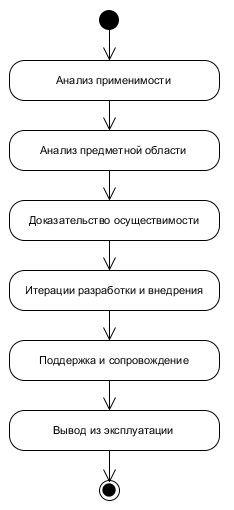
\includegraphics[width=0.25\textwidth]{part3/classicMethodology.png}
		\caption{"`Классическая"' методология разработки визуального предметно-ориентированного языка.}
		\label{classicMethodology}
	\end{center}
\end{figure}

Деятельность на фазе анализа применимости была описана в разделе~\ref{chapterFeasibilityStudy} 
данной работы, её результатом является решение о том, имеет ли смысл применять предметно-ориентированный 
подход для данной ситуации. Этот этап не имеет инструментальной поддержки и требует 
опыта экспертов в предметно-ориентированном подходе.

Анализ предметной области в предлагаемой методологии проводится неформально, согласно 
рекомендациям из~\ref{chapterDomainAnalysis} данной работы. Специальной инструментальной 
поддержки этого этапа в данном случае не предполагается, впрочем, для небольших проектов, 
она и не требуется. Этап анализа предметной области может перекрываться с этапом анализа 
применимости, поскольку для принятия решения о применении DSM-подхода могут требоваться 
знания о предметной области. Этот этап также может перекрываться с первой итерацией 
разработки, поскольку для записи знаний о предметной области может использоваться 
метаредактор (это рекомендуемая практика, набросок метамодели полезен как для понимания 
взаимосвязи основных концепций предметной области, так и как то, из чего может быть 
получен первый прототип редактора языка).

Следующий этап, доказательство осуществимости (proof of concept) является первым этапом 
разработки, и имеет внутреннюю структуру такую же, как одна из итераций следующего этапа, 
итерации разработки и внедрения. Отличие его от последующих итераций в том, что он не 
имеет своей целью реализацию всего, что необходимо, и относительно короток по времени. 
На этом этапе выбирается какой-то узкий срез предметной области и для него строится 
законченное DSM-решение, с редактором, генератором, предметно-ориентированной библиотекой 
и т.д. Задача этого этапа --- убедить будущих пользователей и руководство в применимости 
DSM-подхода, получить раннюю обратную связь, и самим убедиться в осуществимости проекта. 
Результатом должен являться первый ограниченный в функциональности прототип, демонстрирующий, 
тем не менее, все составные части будущего продукта. На основании результатов этого 
этапа может быть принято решение отказаться от продолжения проекта.

Разработка и внедрение состоит из нескольких итераций, порядок действий для каждой 
из которых представлен на рисунке~\ref{classicMethodologyIteration}. Начинается разработка 
с определения метамодели языка с помощью визуального метаязыка, либо внесения изменений 
в уже существующую метамодель. Как только абстрактный синтаксис задан, следующие действия 
можно выполнять параллельно.

\begin{figure} [ht]
	\begin{center}
		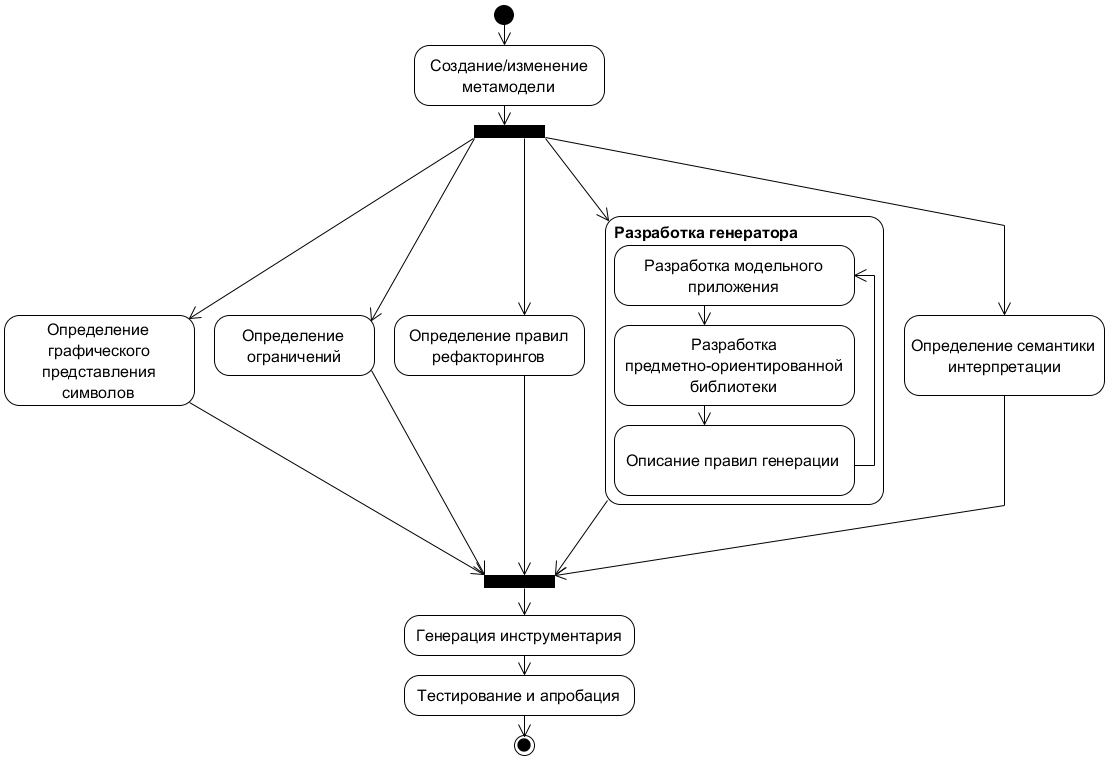
\includegraphics[width=0.9\textwidth]{part3/classicMethodologyIteration.png}
		\caption{Итерация проектирования и разработки языка.}
		\label{classicMethodologyIteration}
	\end{center}
\end{figure}

\begin{enumerate}
	\item Определение графического представления символов языка. Это должно делаться 
		либо в графическом редакторе формы фигур, либо с помощью декларативного текстового
		языка описания формы, DSM-платформа должна минимизировать ручное кодирование. 
		Связано это с тем, что разработку предполагается вести короткими итерациями, и 
		тратить время на кодирование и отладку весьма нежелательно.
	\item Задание ограничений на модели. Здесь речь идёт не про ограничения на состояние 
		создаваемой с помощью DSM-решения системы во время выполнения, а про ограничения 
		на модели, создаваемые при помощи DSM-решения, которые проверяются при рисовании 
		моделей. Ограничения могут быть заданы различными способами, насколько это позволяет
		выбранная для реализации DSM-платформа. В проекте QReal ограничения задаются с помощью 
		визуального языка, при этом модель ограничений отделена от метамодели, и не обязательна 
		для создания редактора. Это позволяет авторам языков не задумываться об ограничениях 
		до тех пор, пока необходимость их использования не станет очевидной.
	\item Определение правил рефакторингов моделей --- довольно редко встречающаяся в 
		DSM-платформах функциональность, но, поскольку автоматизация рефакторингов становится 
		всё более распространённой в текстовых средах разработки, представляется, что 
		скоро и инструменты визуального программирования без рефакторингов будут немыслимы. 
		Простой пример рефакторинга --- вынесение фрагмента диаграммы на языке описания 
		поведения в подпрограмму. Рефакторинги специфичны для конкретных языков, поэтому 
		их необходимо задавать на уровне метамодели, а не поддерживать вручную в DSM-решении. 
		Как и в случае с ограничениями, используемый инструментарий должен позволять не 
		задумываться над рефакторингами без нужды и генерировать инструменты без них. Кроме 
		того, правила задания рефакторингов должны описываться на визуальном предметно-ориентированном 
		языке, опять-таки, по той причине, что при быстром цикле итераций, предполагаемом 
		данной методологией на ручное кодирование тратить усилия нежелательно.
	\item Разработка семантики языка может осуществляться в двух видах, либо путём описания 
		правил интерпретации, либо путём создания генератора в какой-либо текстовый язык. 
		Наиболее часто требуется только порождать по моделям код, и тогда используется 
		генератор, иногда бывает полезно делать и то и другое (например, интерпретатор 
		для интерактивной отладки на уровне модели, и генератор для порождения результирующего 
		кода). Иногда генерировать текстовое представление программы не требуется вовсе 
		(например, в режиме удалённого управления роботом или симуляции на двухмерной 
		модели в примере из раздела~\ref{chapterQRealRobots}). Подходы к заданию этих 
		двух видов описания семантики совершенно разные.
		\begin{enumerate}
			\item Семантика интерпретации, как правило, задаётся в виде правил преобразования 
				графа модели, сродни рефакторингам. Интерпретатор применяет эти правила до 
				тех пор, пока существует хотя бы одно правило, которое он может применить. 
				Правила преобразования могут иметь побочные эффекты, с помощью которых может 
				быть реализовано взаимодействие с внешними компонентами или устройствами, 
				вычисление выражений на текстовом языке, встроенном в визуальный, и даже генерация. 
				Семантика интерпретации должна задаваться на визуальном языке (наиболее удобный 
				формализм для этого --- графовые грамматики
				%TODO: ссылка
				), побочные эффекты могут записываться на текстовом языке.
			\item Разработка генератора в текстовый язык обычно несколько сложнее. Процесс 
				разработки состоит из трёх шагов, как правило, выполняемых итеративно.
				\begin{enumerate}
					\item Разработка модельного приложения. Модельное приложение здесь --- это 
						пример того, что требуется сгенерировать. Писать генератор сразу же, без 
						чёткого понимания, что именно должно быть сгенерировано, очень сложно, 
						поэтому сначала требуется создать пример приложения вручную, и добиться 
						его работоспособности. Пример должен быть простым, но покрывать все разумные 
						случаи, которые могут быть сгенерированы по диаграмме. При этом при написании 
						примера необходимо помнить о том, что его потом придётся генерировать, 
						так что структура программы должна быть удобной для генерации. Для разработки 
						примера используются средства программирования целевой платформы. После 
						того, как приложение отлажено, в DSM-решении рисуется модель, по которой 
						оно могло бы быть сгенерировано.
					\item Когда модельное приложение готово, его части, которые не будут меняться 
						от модели к модели, имеет смысл вынести в отдельную библиотеку или каркас, 
						написанную вручную. Такая библиотека называется библиотекой времени выполнения 
						(runtime) и нужна для того, чтобы упростить написание генератора. Она может 
						быть довольно сложной (вплоть до того, что представлять из себя полноценное 
						приложение, которое лишь конфигурируется результатом генерации), её может 
						вообще не быть (если генерируются достаточно общие приложения, которым 
						достаточно возможностей целевой платформы). Подробнее соображения по разработке 
						предметно-ориентированной библиотеки и балансе функциональности между 
						ней и генератором см. в \cite{kelly2008domain}.
					\item Разработка собственно генератора, как правило, заключается в "`шаблонизации"' 
						готового модельного приложения --- места, параметризуемые информацией из 
						модели, размечаются директивами, руководствуясь которыми генератор формирует 
						целевой код. Конкретный способ задания правил генерации зависит от возможностей 
						DSM-платформы, как правило используется текстовый язык описания правил 
						генерации, либо генератор пишется вручную. В проекте QReal также используется 
						текстовый предметно-ориентированный язык или рукописные генераторы, создание
						графического языка заданий правил генерации представляется интересной областью дальнейших исследований. 
						В процессе разработки генератора часто приходится править модельное приложение, 
						чтобы сделать его структуру более пригодной для генерации, после чего корректировать 
						библиотеку времени выполнения, поэтому процесс разработки генератора итеративен.
				\end{enumerate}
			\end{enumerate}
	\item Следующий шаг, генерация инструментария, должен производиться с возможно меньшим 
		участием человека. Кроме того, генерация должна быть достаточно быстрой, и результат 
		генерации должно быть можно сразу же проверить в среде. Это важно, поскольку тогда 
		результат внесения своих изменений разработчик языка может проверить, ещё помня 
		о них, и не переключая своё внимание на рутинные действия. 
	\item Тестирование и апробация созданных инструментов проводятся сначала разработчиком, 
		затем экспертами предметной области, для которых создаётся язык. Для начальных 
		итераций обычно достаточно наличия одного эксперта, который бы попробовал воспользоваться 
		созданным DSM-решением и высказал замечания, для более поздних итераций требуется 
		расширять базу пользователей и давать им возможность решать реальные практические задачи. 
		Чем раньше это будет сделано, тем быстрее будет получена обратная связь, и тем 
		быстрее можно будет внести коррективы в создаваемый инструментарий или выявить 
		нужную пользователям функциональность, которая пока не была реализована. На этом 
		этапе потребуется сборка инсталляционного пакета для DSM-решения, написание документации, 
		исправление большого количества мелких ошибок, демонстрация инструмента пользователям, 
		наблюдение за их действиями в инструменте, сбор обратной связи. По результатам 
		апробации вносятся необходимые коррективы в концептуальную модель и в метамодель 
		языка, после чего цикл разработки повторяется заново.
\end{enumerate}

Следующий этап, поддержка и сопровождение, включает в себя прежде всего исправление 
ошибок в инструментарии и расширение или корректировку визуального языка. К этому 
моменту основная разработка должна быть завершена, поэтому сопровождение осуществляется 
меньшей командой разработчиков. На этом этапе важным фактором является версионирование 
метамодели вместе с другими исходными кодами DSM-решения, чтобы не допустить ситуации, 
когда изменения в метамодели не согласованы с изменениями в инструментах, которые её 
используют. Кроме того, необходимо следить за совместимостью существующих пользовательских 
моделей с новыми версиями метамодели языка --- пользователи не должны потерять уже 
проделанную работу. Поддержка и сопровождение обычно состоит из коротких циклов внесения 
изменений, подготовки, если требуется, средств миграции моделей на новую версию метамодели, 
подготовку инсталляционного пакета, тестирование и развёртывание новой версии инструментария 
у пользователей. Даже небольшие DSM-решения могут быть используемыми годами, поэтому 
поддержка и сопровождение может быть очень продолжительна по времени.

Вывод из эксплуатации --- заключительная фаза жизненного цикла DSM-решения. Устаревшее 
DSM-решение может быть заменено более новым, может быть произведён реинжиниринг, оно 
может быть просто снято с сопровождения. При этом в любом случае пользователей следует 
заранее оповестить о прекращении поддержки и запланировать дальнейшие действия.

\section{Метамоделирование на лету}
\label{chapter:MetamodelingOnFly}
"`Метамоделирование на лету"' --- новая методология, разработанная в рамках данной 
диссертационной работы, и призванная оптимизировать начальные этапы "`классической"' 
методологии с целью максимально возможно сократить время от принятия решения о реализации 
DSM-решения до получения первого работающего прототипа редактора визуального языка, 
и максимально вовлечь конечного пользователя в процесс разработки. Основной принцип 
данной методологии состоит в том, что создание визуального языка проходит непосредственно 
в процессе рисования диаграммы, без использования метаредактора. Для этого требуется 
специальная поддержка со стороны DSM-платформы, реализация которой в QReal будет описана 
в главе~\ref{chapter:Implementation}:
\begin{enumerate}
	\item интерпретация метамодели, когда редактор не генерируется по метамодели языка, 
		а имеется настраиваемый редактор, который использует внутреннее представление 
		метамодели в памяти для получения информации о языке;
	\item пользовательский интерфейс над интерпретатором метамодели, дающий возможность 
		добавлять элементы, удалять элементы, добавлять, редактировать и удалять свойства 
		элементов, менять графическое представление элементов прямо во время работы.
\end{enumerate}

Основной этап предлагаемой методологии --- прототипирование языка --- начинается сразу 
после этапа анализа применимости, и идейно близка к методологии, изложенной в работе 
\cite{repenning1995agentsheets}. Разработчик языка и будущий пользователь работают 
за одним рабочим местом. При запуске DSM-платформы они видят канву для рисования и 
пустую палитру. Пользователь объясняет, что он примерно хотел бы нарисовать, разработчик 
языка добавляет на палитру новые элементы, определяет для них графическое представление, 
пользователь рисует. Пользователь может сказать, что такой-то элемент должен содержать 
такую-то дополнительную информацию, тогда разработчик добавляет элементу новое свойство, 
задаёт его тип и значение по умолчанию, и пользователь продолжает рисовать диаграмму, 
используя новое свойство. Через некоторое время пользователь может сам добавлять и 
редактировать типы элементов, и работа полностью передаётся ему, разработчик языка 
лишь следит за процессом и консультирует при необходимости пользователя. Работа заканчивается, 
когда модельное приложение полностью нарисовано, после чего текущая интерпретируемая 
метамодель сохраняется в виде, пригодном для дальнейшего редактирования в метаредакторе. 
После этой фазы идут итерации "`классической"' методологии по доработке созданного 
прототипа, дополнению его ограничениями, рефакторингами, интерпретатором и генератором, 
подготовки инсталляционного пакета, развертывания и сбора обратной связи. На этих этапах 
пользователи, как и в "`классической"' модели, непосредственно в разработке не участвуют, 
поскольку этапы гораздо более продолжительны во времени и прямо при пользователе выполнены 
быть не могут.

Модель жизненного цикла языка, использующая "`метамоделирование на лету"', представлена 
на рисунке~\ref{metamodelingOnFly}.

\begin{figure} [ht]
	\begin{center}
		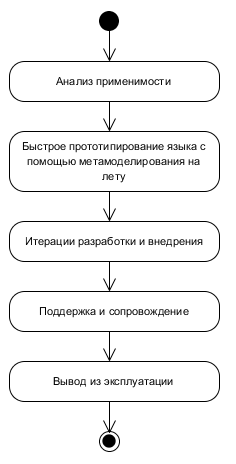
\includegraphics[width=0.25\textwidth]{part3/metamodelingOnFly.png}
		\caption{Методология "`метамоделирования на лету"'.}
		\label{metamodelingOnFly}
	\end{center}
\end{figure}

Здесь не проводится формального или даже неформального анализа предметной области в 
общепринятом понимании, знания о предметной области извлекаются из эксперта прямо 
в процессе прототипирования языка. Также отсутствует фаза доказательства применимости 
(proof of concept), поскольку редактор создаётся прямо на глазах пользователя, и пользователь 
может сразу сказать, то ли это, что он хочет. Разумеется, генератор, предметно-ориентированную 
библиотеку и т.д. придётся писать потом, так что на самом деле proof of concept просто 
смещён на первую итерацию разработки, но по окончании прототипирования по крайней мере 
у одного будущего пользователя DSM-решения есть уверенность в его полезности и применимости 
(причём, довольно сильная, потому что фактически он сам это решение создал).

Все остальные этапы жизненного цикла и деятельности на этих этапах совпадают с аналогичными 
этапами в "`классической"' методологии (поскольку результатом прототипирования будет 
обычная метамодель). Для небольших проектов эта методология наиболее применима, поскольку 
в таком случае всю остальную инструментальную поддержку оказывается возможно реализовать 
за одну-две итерации и получить максимальную выгоду от высокой скорости начального 
прототипирования языка. При этом наиболее эффективна эта методология в том случае, 
если пользователем будущего языка станет сам его разработчик.

Инструментальные средства поддержки метамоделирования на лету не могут быть такими же 
выразительными, как средства, предоставляемые полноценным метаредактором. Связано 
это с тем, что, функциональность метамоделирования на лету должна быть максимально 
простой и легковесной, чтобы ею мог пользоваться эксперт предметной области, не разбирающийся 
в тонкостях создания визуальных языков. По сути эксперт работает с метамоделью языка, 
но не должен подозревать об этом, и тем более не должен владеть связанной с метамоделированием 
терминологией. Метамодель оказывается скрыта от пользователя. Разумеется, полноценный 
синтаксис визуального языка таким образом не задать, простой пример --- указание того, 
к каким узлам может быть подключена связь, было бы слишком сложно для такого режима. 
Поэтому в режиме метамоделирования на лету для метамодели предполагаются разумные умолчания, 
дающие максимальную свободу действий пользователя --- например, связям разрешается соединять 
любые узлы языка. Это допустимо, поскольку при первоначальном прототипировании пользователь 
рисует заведомо "`правильные"' диаграммы, то есть то, что он хочет увидеть. Для полноценного 
решения такой подход недопустим, поскольку пользователи неизбежно будут ошибаться, и 
система должна не давать пользователю совершать ошибок настолько, насколько это возможно. 
Поэтому после быстрого прототипирования требуется правка метамодели языка в метаредакторе 
и внесение в неё дополнительных ограничений. Кроме того, сам язык после быстрого прототипирования 
будет задан не так, как это делалось бы вручную --- без учёта инфраструктурных соображений, 
таких как группировка сущностей языка по пакетам или отношений наследования между элементами. 
Таким образом, чтобы получить сопровождаемую и переиспользуемую метамодель языка, требуется 
рефакторинг полученной после метамоделирования на лету метамодели.

Сформулируем требования к интерфейсу и функциональности режима метамоделирования на лету.
\begin{enumerate}
	\item Вся функциональность метамоделирования на лету должна расширять существующую 
		функциональность редактора диаграмм. С точки зрения интерфейса этот режим должен 
		выглядеть как рисование диаграммы в обычном DSM-решении, с некоторыми дополнительными 
		возможностями.
	\item Должна присутствовать возможность добавить элемент на палитру, задав его имя. 
		При этом для элемента задаётся некоторая форма по умолчанию (например, прямоугольник), 
		элемент создаётся без свойств.
	\item Должна быть возможность задать внешний вид элемента с использованием редактора 
		формы фигур, при этом все уже существующие на диаграмме элементы должны обновить 
		свой внешний вид.
	\item Должна быть возможность удалить элемент из палитры, если его экземпляров нет на диаграмме.
	\item Должна быть возможность создавать копию элемента в палитре. При этом его внешний 
		вид и свойства копируются, после чего могут быть редактируемы независимо.
	\item Должна быть возможность редактировать свойства элементов с палитры.
		\begin{enumerate}
			\item Добавлять новые свойства, задавая им имя, тип и значение по умолчанию. 
				Существующим на диаграмме элементам новые свойства добавляются автоматически, 
				со значением по умолчанию, заданным для этого свойства. Явно значение по умолчанию 
				при добавлении можно не указывать, в таком случае используется значение по 
				умолчанию для типа свойства (например, свойства целочисленного типа инициализируются 
				значением 0). 
			\item Удалять существующие свойства. Если на диаграмме присутствуют элементы с 
				удаляемыми свойствами, выдаётся предупреждение с перечислением элементов, имеющих 
				эти свойства, и свойства просто удаляются с диаграммы, если пользователь согласен.
			\item Редактировать имя, тип и значение по умолчанию существующих свойств. При 
			этом, если изменяется тип свойства элемента, экземпляры которого присутствуют 
			на диаграмме, должно выполняться автоматическое преобразование, если это возможно. 
			Если невозможно (например, строку, содержащую латинские буквы, преобразуют в число), 
			пользователю выдаётся предупреждение с перечислением экземпляров элементов, имеющих 
			такие свойства.
		\end{enumerate}
	\item Практически никакие ограничения на рисуемые в этом режиме диаграммы не накладываются 
		(за исключением ограничений, присущих самой среде). Любая связь может быт подключена 
		к любому элементу, любой элемент может содержаться в любом другом элементе. Корректность 
		значений свойств элементов проверяется с точки зрения типа свойства, дополнительные 
		ограничения на значения свойств в этом режиме не накладываются.
	\item Метамодель, полученную в режиме метамоделирования на лету, должно быть можно 
		открыть и редактировать в метаредакторе. Метамодель должна быть "`плоской"' в том 
		смысле, что система не должна делать предположений о структуре и иерархической 
		организации метамодели. Даже в том случае, когда применялось копирование элемента, 
		копия и оригинал не должны быть связаны. Структурирование модели проводится отдельным 
		этапом, в метаредакторе, по окончании быстрого прототипирования.
\end{enumerate}

Перечисленные требования до некоторой степени поддержаны в DSM-платформе MetaEdit+ 
(\cite{kelly2008domain}), там имеется возможность прямо в процессе моделирования менять 
внешний вид и свойства элемента. При этом для того, чтобы добавить или удалить элемент, 
необходимо воспользоваться редактором метамодели, так что это не может быть легко 
сделано самим экспертом без помощи человека, умеющего пользоваться этим инструментом, 
поэтому можно утверждать, что MetaEdit+ не может быть в полной мере использован как 
DSM-платформа, поддерживающая данную методологию. Ближе всего к данной методологии 
методология, предлагаемая инструментом Agentsheets (\cite{repenning1995agentsheets}), 
она тоже позволяет работать непосредственно с пользователем и очень быстро создавать 
визуальные языки (даже с поддержкой интерпретации). Однако, во-первых, технология 
предполагает программирование на текстовом языке, что делает невозможным её использование 
без помощи специалиста по созданию языка, во-вторых, она не предполагает доработки метамодели 
в полноценном метаредакторе, поэтому применима в более узком наборе случаев, чем типичные 
DSM-платформы, и плохо масштабируется на большие проекты.

